\documentclass{beamer}

\mode<presentation>{
  \usetheme{Warsaw}
  \setbeamercovered{transparent}
}

\usepackage[english]{babel}
\usepackage[latin1]{inputenc}
\usepackage{times}
\usepackage[T1]{fontenc}
\usepackage{subfigure}

\usepackage{algorithm}
\usepackage{algorithmic}

%%%%%%%%%%%%%%%%%%%%%%%%%%%%%%%%%%%%%%%%%%%%%%%%%%%%%%%%%%%%
\title{Title}

\author{First AUTHOR$^{(1)}$ and Second AUTHOR$^{(2)}$}

\institute{
{\tiny  First Institution\\
  (1) first@mail\\
  ~\\
  Second Institution\\
  (2) another@mail.fr\\
}
}

\date[ABREV]{When ...\\
 {\footnotesize At ...}}

\pgfdeclareimage[height=0.8cm]{le-logo}{liasd}
\logo{\pgfuseimage{le-logo}}

\AtBeginSection[]{
  \begin{frame}<beamer>{Outline}
    \tableofcontents[currentsection]
  \end{frame}
}

%%%%%%%%%%%%%%%%%%%%%%%%%%%%%%%%%%%%%%%%%%%%%%%%%%%%%%%%%%%%
\begin{document}

\begin{frame}
  \titlepage
\end{frame}

\begin{frame}{Outline}
  \tableofcontents
\end{frame}

%%%%%%%%%%%%%%%%%%%%%%%%%%%%%%%%%%%%%%%%%%%%%%%%%%%%%%%%%%%%
\section{Introduction}
\begin{frame}
  \begin{exampleblock}{(Situation or used env)}
    \begin{itemize}
    \item Motions, single agent behaviors, collective behaviors
    \item Competiting 11 vs 11 in simulation (3DSSL RoboCup competition)
    \end{itemize}
  \end{exampleblock}
  
  \begin{alertblock}{(Problem or questions)}
    \begin{itemize}
    \item Different positions
    \item Different roles and skills
    \item Different optimizations
    \item Different characteristics ?
    \end{itemize}
  \end{alertblock}
\end{frame}

%%%%%%%%%%%%%%%%%%%%%%%%%%%%%%%%%%%%%%%%%%%%%%%%%%%%%%%%%%%%
\section{Related Work}
\begin{frame}
  \begin{itemize}
  \item References ...
  \end{itemize}
\end{frame}

%%%%%%%%%%%%%%%%%%%%%%%%%%%%%%%%%%%%%%%%%%%%%%%%%%%%%%%%%%%%
\section{Optimization process}

\begin{frame}
  ~\\
  \footnotesize{
    According to $n$ trials with $p$ parameters :\\
    ~~~$s$~~: success\_rate of 1 trial\\
    ~~~$\nu$~~: averages and standard deviations (\emph{i.e.} results) of 1 trial\\
    ~~~$\nu'$ : best acceptable results\\
    ~~~$h$~~: quality of the results ($ACCEPT$, $EQUIVALENT$ or $REJECT$)\\
    ${\cal{H}}$ : history set that regroups ($p$, $h$) pairs\\
    ${\cal{L}}$ : parameters bound\\
  }
  \begin{algorithm}[H]
    \algsetup{linenosize=\tiny}
    \scriptsize
    \begin{algorithmic}[1]
\STATE ($\nu'$, ${\cal{H}}$) $\leftarrow$ ($\emptyset$, $\emptyset$)
\FOR{$i=0$ to $n$}
\STATE $p \leftarrow$ {\tt newParams} (${\cal{H}}$, ${\cal{L}}$)
\STATE ($s$, $\nu$) $\leftarrow$ {\tt performTrial} ($p$)
\STATE ($\nu'$, $h$) $\leftarrow$ {\tt pickOut} ($s$, $\nu$, $\nu'$)
\STATE {\tt insert} (($p$ , $h$), ${\cal{H}}$)
\ENDFOR
\STATE {\bf return} {\tt paramsFrom} ($\nu'$)
    \end{algorithmic}
    \caption{{\tt evolving} ($n$, ${\cal{L}}$, {\tt pickOut})}
  \end{algorithm}

\end{frame}


%%%%%%%%%%%%%%%%%%%%%%%%%%%%%%%%%%%%%%%%%%%%%%%%%%%%%%%%%%%%
\section{Experiments}

\begin{frame}
\begin{footnotesize}
\begin{table}[h]
\centering
\caption{{\tt pickOut} decision parameters}
\label{tabExp}
\begin{tabular}{|p{3cm}|p{1cm}|}
\hline
$SUCCESS\_RATE$ & 0.75 \\
\hline
$XY\_RATIO$ & 0.25 \\
\hline
$\alpha$ & 3.0 \\
\hline
$\beta$ & 1.0 \\
\hline
$\gamma$ & 0.7 \\
\hline
\end{tabular}
\end{table}
\end{footnotesize}
\end{frame}

\begin{frame}
  \begin{figure}[!t]
    \centering
    \subfigure[Default]{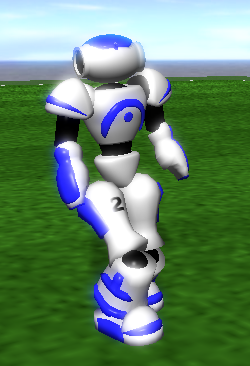
\includegraphics[scale=0.33]{figure/optim1.png}}\quad
    \subfigure[Optim.1]{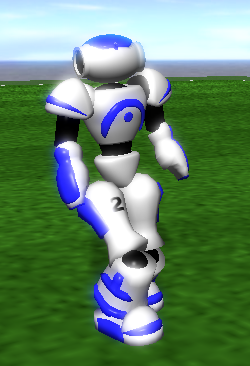
\includegraphics[scale=0.33]{figure/optim1.png}}\quad
    \subfigure[Optim.2]{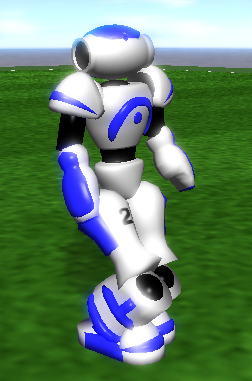
\includegraphics[scale=0.32]{figure/optim2.png}}
    \caption{Three resulting NAO profiles}
    \label{fig3}
  \end{figure}
\end{frame}

%%%%%%%%%%%%%%%%%%%%%%%%%%%%%%%%%%%%%%%%%%%%%%%%%%%%%%%%%%%%
\section{Conclusion}
\begin{frame}
  \begin{itemize}
  \item Few points to conclude
  \item ...
  \end{itemize}
\end{frame}

%%%%%%%%%%%%%%%%%%%%%%%%%%%%%%%%%%%%%%%%%%%%%%%%%%%%%%%%%%%%
\begin{frame}
  \titlepage
\end{frame}

\begin{frame}
\begin{columns}
\begin{column}{.56\textwidth}
\footnotesize{Checking NAO's model proper sizing:
\begin{itemize}
\item $ThighRelHip2\_Z$ : relative distance between hip and thigh center of mass
\item ( $ThighRelHip2\_Z$ value is $-0.04[m]$ )
\item From $-0.01$ to $-0.10[m]$ 
\end{itemize}
Experiment over $500$ iterations:
\begin{itemize}
\item $REJECT$ represented in black
\item $EQUIVALENT$ represented in gray
\item $ACCEPT$ represented in white
\item $Optim.2$ value is $-0.038[m]$
\end{itemize}
}
\end{column}%
\hfill%
\begin{column}{.45\textwidth}
    \begin{figure}[!t]
      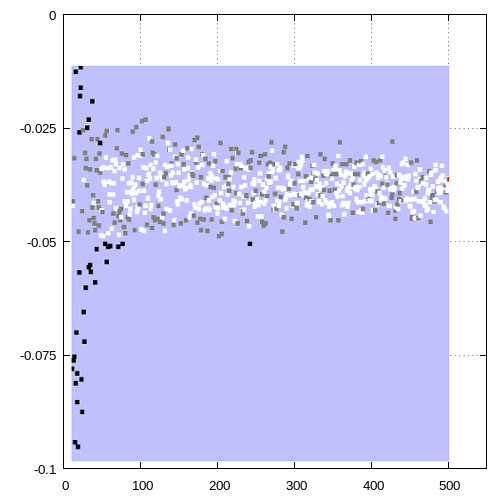
\includegraphics[scale=0.28]{figure/img1-grid.png}
      \label{fig4}
    \end{figure}
\end{column}%
\end{columns}
\end{frame}

\begin{frame}
\footnotesize{
Two parameters important in human morphology:
\begin{itemize}
\item $ThighRelHip2\_Z$: semi-length of the femur
\item $ratio\_flexion$: hip height over total leg's length
\end{itemize}
Three general parameters to adjust the walk: 
\begin{itemize}
\item $long\_offset\_MidAnkles\_2\_Torso\_Init$: horizontal distance between ankles' middle and torso center
\item $height\_lift$: maximal height of lef lift-off
\item $xlength\_step\_max$: maximal step length
\end{itemize}
}
\end{frame}

\end{document}


